\chapter{Le modèle en couches}
\section{Introduction}
Le but de ce modèle est de décrire les propriétés des états fondamentaux (spin, parité, moments dipolaire, 
quadrupolaires, \dots). Il a aussi pour but d'expliquer l'orgine des nombres magiques ($2,8/,20,2/8,50,82,126)$. 
Ceux-ci ont des propriétés intéressantes
\begin{itemize}
\item[$\bullet$] Nombre de neutrons/protons donnant des propriétés particulières au noyau
\item[$\bullet$] Grande énergie de liaison et énergie d'excitation élevée
\item[$\bullet$] Effets microscopiques (absents des modèles collectifs) et petit rayon
\end{itemize}

L'Hamiltonien exact s'écrit
\begin{equation}
H = \sum_{i=1}^A T_i +\sum_{i=1}^A\underbrace{\sum_{j=1}^A v(r_i-r_j)}_{\approx U_i(r_i)}
\end{equation}
Celui-ci est alors remplacé par
\begin{equation}
H = \sum_{i=1}^A (T_i+U_i(r_i)) + H_{res}
\end{equation}
où $H_{res}$ est un Hamiltonien "résiduel" supposé négligeable. Cet Hamiltonien est à particules indépendantes et
chaque nucléon ressent un potentiel moyen généré par les autres nucléons. En négligeant le terme résiduel, nous
avons la forme d'un Hamiltonien séparable : le problème à $A$ nucléons a été changé en $A$ problèmes à $1$ 
nucléon
\begin{equation}
H = \sum_{i=1}^A H_i,\qquad\qquad E = \sum_{i=1}^A E_i, \qquad\qquad \Psi = \Phi_1\dots\Phi_A
\end{equation}

Différentes approximations sont possibles pour le potentiel $U(r_i)$. Par exemple, l'interaction de \textsc{Coulomb}
étant faible par apport à l'interaction nucléaire, nous allons négliger \textsc{Coulomb}. Généralement, $U_i$ tend
alors vers zéro et tend à être attractif à courte portée (forme typique d'un potentiel nucléaire). Mais un tel
potentiel n'ayant pas de solution analytique, il va falloir ruser.


\subsection{A. L'oscillateur harmonique}
Dans le cas d'un oscillateur à une dimension $x$, nous avons $U(x) = \frac{1}{2}m\omega^2x^2$. On peut écrire
\begin{equation}
\left(\frac{\hbar^2}{2m}\frac{d^2}{dx^2} + \frac{1}{2}m\omega^2x^2\right)\phi(x) = E\phi(x)\quad\Leftrightarrow
\quad \left(-\frac{d^2}{dx^2}-\frac{m\omega^2}{\hbar^2}x^2\right)\phi(x) = \frac{2mE}{\hbar^2}\phi(x)
\end{equation}
On peut trouver $b^4 = \hbar^2/(m^2\omega^2)$ (où $b$ est le paramètre d'oscillateur). En posant
\begin{equation}
\phi(x) = \exp(-x^2/2b^2)\tilde{\phi}(x)
\end{equation}
On peut trouver les énergies et les fonctions propres
\begin{equation}
E_n(x) = \hbar\omega\left(n+\frac{1}{2}\right),\qquad\qquad \phi_n(x) \propto \exp(-x^2/2b^2) H_n(x/b)
\end{equation}
où $H_n(x)$ sont les polynômes d'\textsc{Hermitte}.

\begin{center}
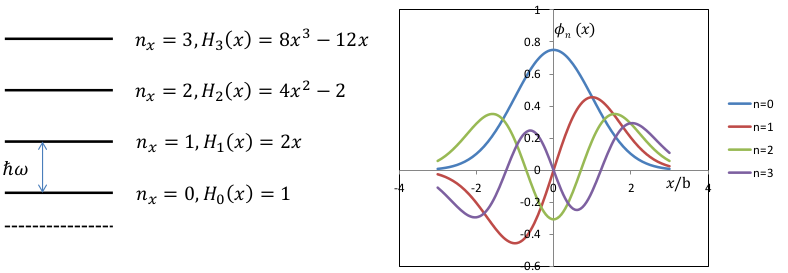
\includegraphics[scale=0.5]{ch9/image1}
\captionof{figure}{ }
\end{center}

La chose fantastique est que le passage en trois 
dimension se fait en sommant les hamiltonien pour chaque dimension. L'énergie est alors donnée par
\begin{equation}
E_{n_x,n_y,n_z} = \hbar\omega\left(n_x+n_y+n_z+\frac{3}{2}\right)
\end{equation}
Pour $n_x=n_y=n_z=0$ il n'existe qu'un seul état possible. Par contre, si l'un deux vaut 1 nous avons
trois états possible. Ceci est la dégénérescence des états, la même énergie est commune à un certain nombre
d'états différents.\\



La dégénérescence (valant toujours 1 dans le cas 1D) est donnée par
\begin{equation}
N_n = \sum_{n_x=0} (n-n_x+1) = \frac{(n+1)(n+2)}{2}
\end{equation}

Les \textit{slides 18} et \textit{19} reprennent ces résultats dans le cas des coordonnées sphériques. On retrouve
au final trois fonctions d'ondes aux coordonnées sphériques qui correspondent aux trois trouvées dans les
coordonnées cartésiennes.\\

	\begin{wrapfigure}[9]{l}{8.5cm}
	\vspace{-5mm}
	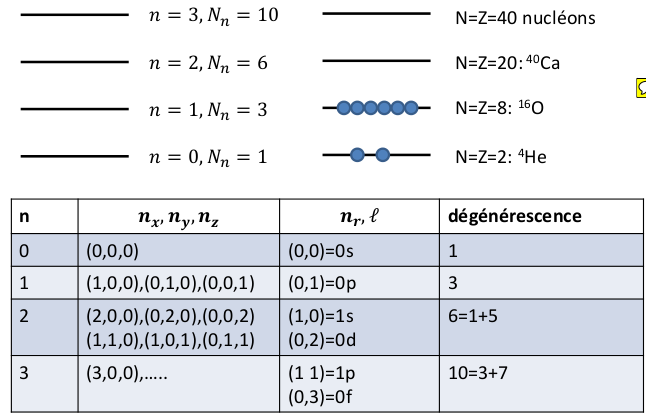
\includegraphics[scale=0.35]{ch9/image2}
	\captionof{table}{ }
	\end{wrapfigure}

Cette dégénérescence compte le nombre de nucléon que l'on peut mettre par niveau. Sur le niveau 0 on peut en
mettre 2, sur le niveau 1 on peut en mettre 6, \dots Il y a chaque fois un facteur deux venant du spin. Si
l'énergie de liaison est grande, c'est parce qu'une couche est fermée : on retrouve bien 2 le premier nombre 
magique (qui correspond à une couche pleine). \\

En effet, si une couche est remplie, rien ne se passera si l'énergie de liaison n'est pas fournie : nombre 
magique. Par contre, si la couche n'est pas remplie il peut y avoir réorganisation au sein de celle-ci. Ce 
modèle permet d'expliquer les trois premiers nombres magiques (2,8,20) grâce à cette explication mais plus les
suivants (40 est prédit comme nombre magique dans cette théorie mais ça ne colle pas expérimentalement). Il 
manque donc quelque chose à ce modèle!

\subsection{B. Puits infini}